\documentclass[11pt]{article}
\usepackage[margin=1in]{geometry}
\usepackage{amsmath}
\usepackage{amssymb}
\usepackage{booktabs}
\usepackage{float}
\usepackage{graphicx}
\usepackage{listings}
\usepackage{xcolor}
\usepackage[hidelinks]{hyperref}
\newcommand{\pra}{\mathrm{PRA}}
\newcommand{\refhandle}{\mathrm{REF}}
\newcommand{\kv}{\mathrm{KV}}
\newcommand{\q}{\mathbf{Q}}
\newcommand{\kmat}{\mathbf{K}}
\newcommand{\vmat}{\mathbf{V}}

\setlength{\emergencystretch}{3em}
\lstset{basicstyle=\ttfamily\small,breaklines=true,frame=single,columns=fullflexible}

\title{Iterative Progressive Retrieval Attention:\\
Bounded Associative Closure over Latent Gist Memory}
\author{Jorge Simao\\EInnovator R\&D -- Center for the Sciences of Computation, Cognition, and Complexity}
\date{\today}
\hypersetup{pdftitle={Iterative Progressive Retrieval Attention},pdfauthor={Jorge Simao}}

\begin{document}
\maketitle

\begin{abstract}
One-shot semantic retrieval finds memory nearest to the current query.  It can miss a second
piece of evidence that is weakly related to the query but strongly related to the first piece.
We study iterative Progressive Retrieval Attention (PRA), which treats cached routing gists as an
implicit graph: the query retrieves a bounded frontier, retrieved gists query the same layer-local
index, and only the final closure is mapped to full native key/value (K/V) state.  The transformer
is not rerun between retrieval rounds.

A parameter-free implementation enforces depth, branch, beam, and unique-chunk budgets; prevents
cycles; retains alternate discovery edges; and emits a versioned retrieval graph before K/V
materialization.  At matched final chunk budgets, controlled two- and three-hop latent graphs
show the intended separation: iterative routing completes every chain over 320 paired trials,
whereas one-shot Top-$B$ retrieves only the first node.  On five independently trained semantic
routers and held-out Qwen3-0.6B features, the result is mixed.  At 10\% selected chunks,
HotpotQA evidence-group completion rises from 0.138 to 0.150/0.163/0.175 for depths 2/3/4, but
any-evidence recall falls from 0.700 to 0.663/0.663/0.613.  QASPER, a mostly direct-evidence
control, favors one-shot routing.  Search comparisons increase by 4.4$\times$ on HotpotQA and
9.8$\times$ on QASPER at depth 2.  Root anchoring reduces drift, and no tested parameter-free
state or path update provides a consistent advantage.  The findings establish the mechanism and
its systems contract, but do not establish that a router trained only for query--evidence
relevance learns a useful evidence--evidence graph.  Associative-edge supervision is the next
test; learned recursion is not yet justified.
\end{abstract}

\section{Introduction}

Suppose a question is directly related to memory chunk $A$.  Chunk $A$, in turn, identifies an
entity or relation needed to find chunk $B$.  A one-shot router computes similarities from the
question to all chunks.  It can retrieve $A$ while missing $B$ because the question does not yet
contain the intermediate relation.  Increasing top-$k$ may find $B$, but it spends the same extra
budget on unrelated chunks.  The problem is not transformer reasoning after evidence arrives.
It is evidence discovery before full memory becomes active.

PRA already separates compact semantic routing state from full layer-native K/V payloads
\cite{simao2026pra,simao2026position,simao2026hf}.  This separation suggests a narrow extension.
After retrieving $A$, use $A$'s compact gist as another query.  Continue for a bounded number of
rounds, preserve the discovery graph, and materialize exact K/V only once.  The resulting path
$q\rightarrow A\rightarrow B$ is explicit.  It does not require another language-model pass,
an intermediate text answer, or serialization through an external tool API.

This paper asks whether pretrained hidden-state gists already possess enough transitive semantic
geometry for that extension to help.  The question has a strict baseline: iterative closure must
beat one-shot Top-$B$ at the same final unique-chunk budget $B$.  Otherwise, retrieval depth adds
cost without adding a useful primitive.

The contributions are fourfold.  First, we formulate iterative PRA as query-conditioned bounded
associative closure over an implicit latent graph.  Second, we implement Level-1 gist-to-gist and
Level-2 aggregate-frontier traversal with deterministic budgets, cycle handling, root anchoring,
transparent path scores, and a versioned graph artifact.  Third, we evaluate five semantic-router
seeds on held-out HotpotQA and QASPER features, together with exact two- and three-hop synthetic
controls.  Fourth, we report a result that narrows the next experiment: traversal works when
associative edges are present, but a router trained for query--evidence ranking does not reliably
induce those edges on natural data.

\section{From Nearest Neighbors to Associative Closure}

\subsection{Why one-shot retrieval can stop too early}

Let $G=\{g_1,\ldots,g_N\}$ be compact routing gists at one transformer layer and let $q$ be the
current routing query.  One-shot PRA returns
\begin{equation}
  N_B(q)=\operatorname{TopB}_{g\in G}\;s(q,g),
\end{equation}
where $s$ is cosine similarity in the learned semantic space.  This operation is appropriate
when every useful chunk is independently similar to $q$.  It is incomplete when
\begin{equation}
  s(q,g_A)\gg 0,\qquad s(q,g_B)\approx 0,\qquad s(g_A,g_B)\gg 0.
\end{equation}
Here $A$ is an entry point and $B$ is relationally accessible only after $A$ is known.

We interpret each chunk as a node in an implicit graph.  High gist similarity supplies candidate
directed edges, generated lazily when a node becomes part of the frontier.  No $N\times N$
adjacency matrix is built.  Iterative PRA therefore computes a bounded semantic neighborhood,
not a proof and not complete reasoning.

\subsection{The complete data path}

Figure~\ref{fig:mechanism} separates traversal from payload activation.  This boundary is the
main systems invariant: compact gists may participate in several search rounds, while full K/V
cannot enter attention until the closure stops.

\begin{figure}[H]
\centering
\fbox{\begin{minipage}{0.92\linewidth}
\centering
\textbf{ONE SHOT}\quad $q\rightarrow\{A,X,Y\}\rightarrow$ full native K/V\\[8pt]
\textbf{ITERATIVE ASSOCIATIVE CLOSURE}\\[3pt]
$q\rightarrow A\rightarrow B\rightarrow C$\\[-2pt]
\hspace{31mm}$\searrow D$\\[5pt]
$\{A,B,C,D\}$ bounded by $B,D,k,$ and beam size\\
$\downarrow$\\
final chunk identities $\rightarrow$ layer-local full native K/V $\rightarrow$ transformer\\[5pt]
\hrulefill\\[-2pt]
\textit{Future Paper 3 interface:} closure graph $\dashrightarrow$ progressive detail allocation
\end{minipage}}
\caption{Iterative PRA increases search depth without transformer reruns.  Gists are routing
state; native K/V is the payload.  The dashed handoff preserves graph signals for later work on
partial materialization.}
\label{fig:mechanism}
\end{figure}

\section{Method}

\subsection{Bounded frontier expansion}

The root query initializes frontier $F_0=\{q\}$ and the visited set is empty.  At round $t$, each
frontier vector proposes its $k$ highest-scoring unseen chunks.  Duplicate proposals are merged,
the best path to each candidate is retained, and at most the remaining beam and unique-node
budgets are accepted.  Accepted gists form $F_t$.  Traversal stops at fixed depth $D$, final
budget $B$, no-new-node convergence, or an optional confidence threshold.

To limit semantic drift, candidate $c$ is scored against both the root and its frontier parent:
\begin{equation}
  e_t(c)=\alpha s(q,g_c)+(1-\alpha)s(f_{t-1},g_c),
  \qquad 0\leq\alpha\leq1.
\end{equation}
At $\alpha=0$, traversal follows local gist edges.  At $\alpha=1$, every round reproduces root
ranking after visited-node removal.  Intermediate values preserve the original information need
while allowing a retrieved node to redirect search.

The primary path score multiplies affinities $a_i=(e_i+1)/2$ along a path:
\begin{equation}
  P(c_t)=\prod_{i=1}^{t}a_i.
\end{equation}
We also evaluate log-sum, final-edge, minimum-edge, mean-edge, and direct-root scores.  These
choices are deliberately transparent.  A learned controller would confound the first question:
whether useful graph structure is already present.

\begin{lstlisting}[caption={Level-1 bounded associative closure},label={alg:closure}]
frontier = {root}; selected = {}; graph = empty
for hop in 1..D:
    proposals = union topk_unseen(parent, G, k) for parent in frontier
    merge duplicate targets; retain parent edges and best path
    accepted = top(proposals, min(beam, B - len(selected)))
    add accepted nodes and edges to graph
    frontier = winning_gists(accepted)
    stop if frontier is empty or len(selected) == B
materialize_full_native_kv(selected)  # only after closure
\end{lstlisting}

\subsection{Level-2 frontier updates}

Direct Level-1 traversal uses each winning gist as the next query.  We compare three
parameter-free updates.  A residual update keeps parent state,
\begin{equation}
 r_{t+1}=\operatorname{normalize}(r_t+\beta g_t),
\end{equation}
while mean and path-weighted mean collapse accepted branches to one aggregate vector and add the
root.  These updates test whether mild state accumulation reduces drift.  They do not rerun a
transformer and introduce no learned parameters.

\subsection{Budgets, cycles, and layer locality}

Four controls bound expansion: depth $D$, neighbors per frontier node $k$, per-round beam size,
and maximum unique chunks $B$.  A visited set prevents $A\rightarrow B\rightarrow A$ from
consuming budget twice.  Alternate parents remain graph edges even when one path wins pruning.
Every index is layer-local.  A query, gist, and native payload from different layers are never
treated as interchangeable merely because their dimensions match.

If $C$ is the number of chunks and $|F_t|$ the frontier size, Level-1 scoring performs
$C\sum_t|F_t|$ gist comparisons.  Full K/V transfer remains proportional to the final selected
payload, exactly as in matched one-shot PRA.  The method trades more compact-index work for a
chance to find a better closure without increasing active K/V.

\section{Experimental Design}

\subsection{Frozen semantic geometry}

We reuse Paper 2's frozen Qwen3-0.6B feature artifact and its attention-input hidden-state
representation \cite{qwen2025qwen3,simao2026hf}.  The held-out split contains 16 HotpotQA and
16 QASPER examples, 32-token chunks, exact evidence-overlap masks, and 1,024-dimensional root and
memory features \cite{yang2018hotpotqa,dasigi2021qasper}.  Five asymmetric linear projections,
each with 262,144 parameters and seeds 11, 23, 37, 53, and 71, map query and memory features to
128 dimensions.  They were trained on the disjoint Paper 2 train split with exhaustive negatives.
No router is trained or selected on iterative results.

The primary setting uses direct frontier gists, multiplicative path score, $\alpha=0.25$, and
$D\in\{2,3,4\}$.  Final budgets are 5, 10, 20, and 30\% of each example's candidate chunks.
One-shot always receives the identical final $B$.  We separately sweep
$\alpha\in\{0,.25,.5,.75,1\}$, all Level-2 updates, and all six path scores at $D=2$, 10\%.

\subsection{What the evidence metrics mean}

Any-evidence recall asks whether one annotated chunk is selected.  Exact all-evidence recall asks
whether every evidence-overlapping 32-token chunk is selected.  Because one supporting sentence
can cross a chunk boundary, we additionally group contiguous positive chunks and define chain
completion as selecting at least one chunk from every group.  The artifact reports budget
feasibility for both definitions.  Hotpot groups are ordered by source position; they are not
claimed to encode causal hop order.  QASPER usually has one contiguous evidence group and is
therefore a direct-retrieval control.

The synthetic controls provide exact causal chains.  Their root is similar to node $A$; each next
node is similar to its predecessor but is outranked from the root by distractors.  At matched
$B=2$ or $3$, one-shot can afford the entry node but not the full chain.  We run 64 examples per
seed for each chain length, yielding 320 paired trials per task.

\subsection{Downstream execution validation}

A separate two-example CUDA smoke loads the pinned Qwen model, indexes one HotpotQA and one
QASPER source, and compares no memory, one-shot, and $D=2$ closure.  One-shot and closure both
request three chunks and materialize 96 native K/V tokens.  This run validates execution and
budget invariants; two examples cannot estimate answer quality.

\section{Results}

\subsection{Exact latent chains validate the mechanism}

Table~\ref{tab:synthetic} gives the cleanest mechanism test.  Both methods find some evidence,
but one-shot retrieves only the entry node.  Iterative traversal follows the designed edges and
completes every chain.  The gain costs one complete index scan per hop.

\begin{table}[H]
\centering
\caption{Matched-budget synthetic results over five seeds and 64 examples per seed.}
\label{tab:synthetic}
\begin{tabular}{llrrrr}
\toprule
Task & Method & Any & Exact chain & Coverage & Comparisons \\
\midrule
2-hop & One-shot Top-2 & 1.000 & 0.000 & 0.500 & 10 \\
2-hop & Iterative $D=2$ & 1.000 & 1.000 & 1.000 & 20 \\
3-hop & One-shot Top-3 & 1.000 & 0.000 & 0.333 & 11 \\
3-hop & Iterative $D=3$ & 1.000 & 1.000 & 1.000 & 33 \\
\bottomrule
\end{tabular}
\end{table}

This result establishes that the implementation can recover indirect nodes without transformer
updates.  It does not show that a pretrained semantic router supplies the required edges.

\subsection{HotpotQA shows a small chain signal and a larger drift cost}

Figure~\ref{fig:hotpot} and Table~\ref{tab:primary} compare natural-data routing.  At 10\%,
one-shot any-evidence recall is $0.700\pm0.065$ (five-seed 95\% interval), while $D=2$ obtains
$0.663\pm0.118$.  Yet group-level chain completion rises from 0.138 to 0.150, and reaches 0.175
at $D=4$.  The two metrics describe different behavior: closure sometimes reaches another
evidence group, but also leaves an easily retrieved entry neighborhood.

\begin{figure}[H]
\centering
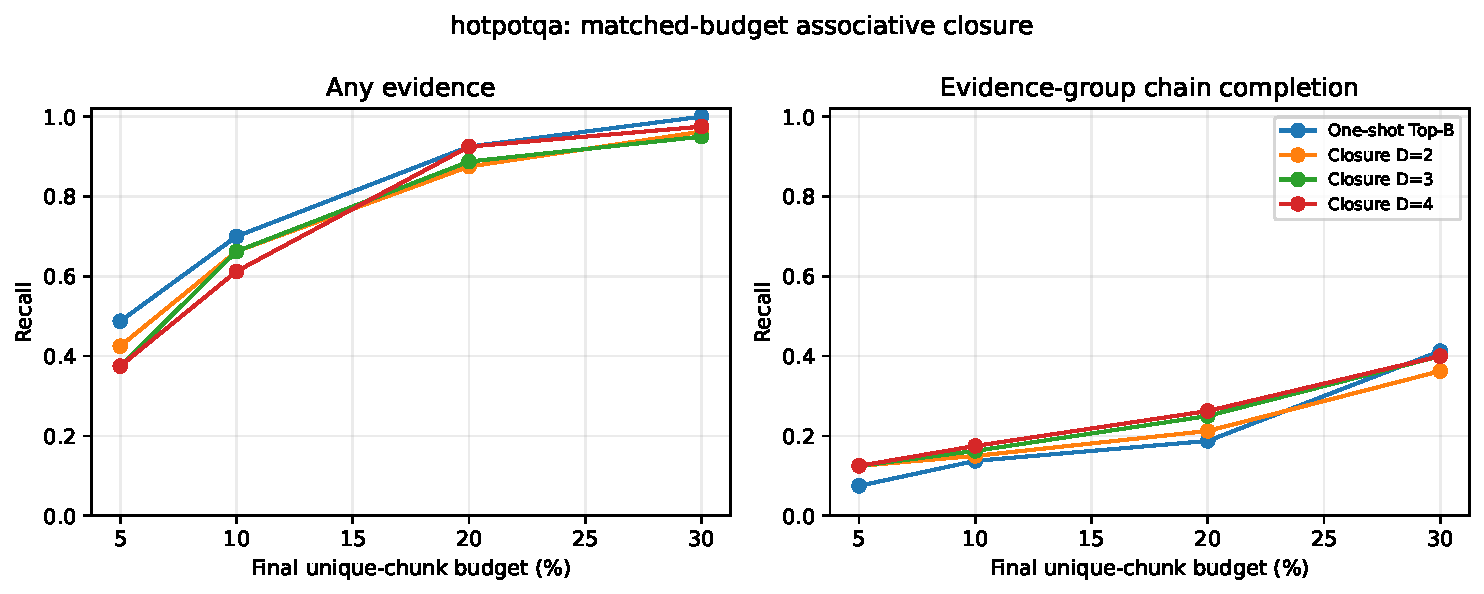
\includegraphics[width=0.92\linewidth]{../shared/results/paper2_5_iterative_pra/hotpotqa_closure_recall.pdf}
\caption{Five-seed HotpotQA matched-budget curves.  Deeper closure modestly improves chain
completion at some sparse budgets but does not improve the broader any-evidence curve.}
\label{fig:hotpot}
\end{figure}

\begin{table}[H]
\centering
\caption{Primary 10\% matched-budget results.  Means combine 16 examples and five independently
trained routers.  ``All'' requires every positive chunk; ``Chain'' requires every evidence group.}
\label{tab:primary}
\begin{tabular}{llrrrrr}
\toprule
Dataset & Method & Any & Chain & All & Coverage & Comparisons \\
\midrule
HotpotQA & One-shot & .700 & .138 & .013 & .207 & 50.1 \\
HotpotQA & Closure $D=2$ & .663 & .150 & .000 & .202 & 219.6 \\
HotpotQA & Closure $D=3$ & .663 & .163 & .000 & .205 & 273.0 \\
HotpotQA & Closure $D=4$ & .613 & .175 & .000 & .193 & 303.2 \\
QASPER & One-shot & .963 & .963 & .213 & .477 & 142.6 \\
QASPER & Closure $D=2$ & .875 & .875 & .200 & .466 & 1395.9 \\
QASPER & Closure $D=3$ & .788 & .788 & .175 & .425 & 1822.1 \\
QASPER & Closure $D=4$ & .825 & .825 & .150 & .426 & 2144.2 \\
\bottomrule
\end{tabular}
\end{table}

At 20\%, Hotpot chain completion rises from 0.188 one-shot to 0.212, 0.250, and 0.263 at depths
2--4.  At 30\%, one-shot returns to the lead (0.412 versus 0.362--0.400).  The effect is therefore
small, budget dependent, and not accompanied by improved exact all-chunk recall.  Five seeds are
insufficient to claim a reliable improvement; the direction also changes with budget.

\subsection{QASPER behaves as a direct-retrieval control}

QASPER's evidence commonly forms one contiguous group, so chain completion equals any-evidence
recall in this protocol.  Figure~\ref{fig:qasper} shows that one-shot dominates throughout the
sparse region.  At 10\%, its any/chain recall is $0.963\pm0.069$ versus $0.875\pm0.095$ for
$D=2$.  Closure adds no useful intermediate relation when the root already addresses the target.

\begin{figure}[H]
\centering
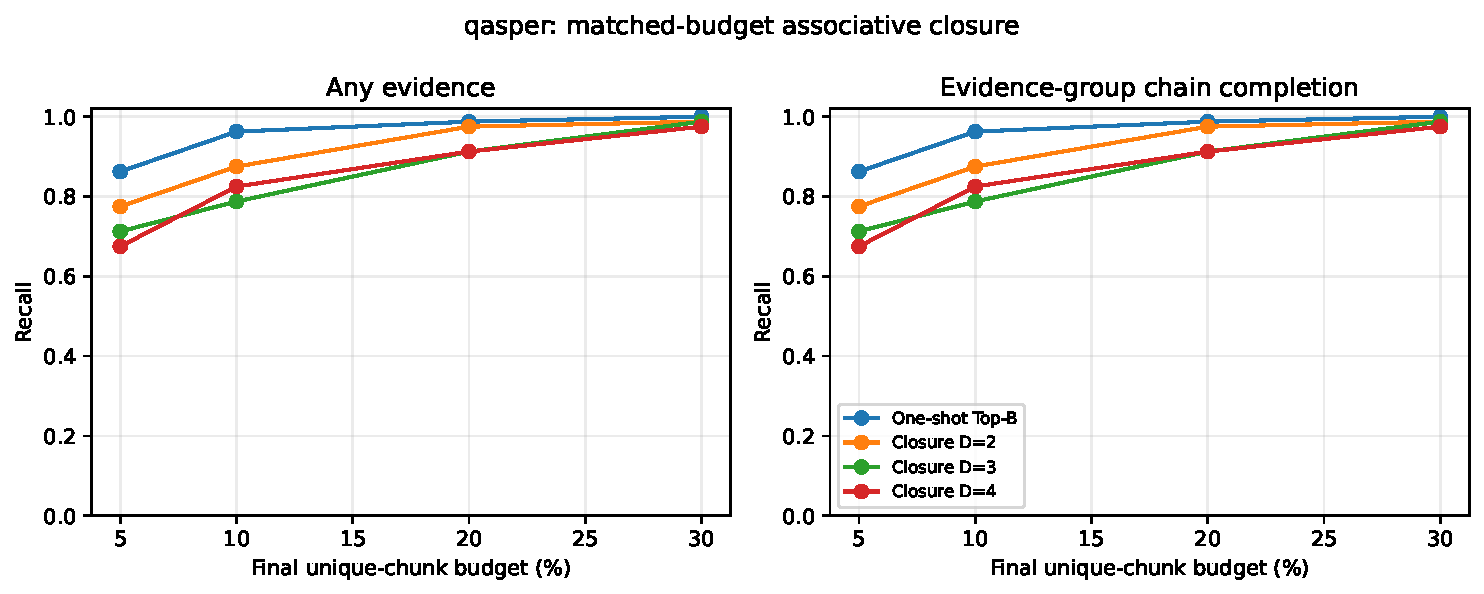
\includegraphics[width=0.92\linewidth]{../shared/results/paper2_5_iterative_pra/qasper_closure_recall.pdf}
\caption{QASPER matched-budget curves.  The mostly single-group evidence protocol favors direct
one-shot ranking, as expected if recursion is unnecessary.}
\label{fig:qasper}
\end{figure}

\subsection{Root anchoring exposes semantic drift}

At 10\% Hotpot, pure local traversal ($\alpha=0$) yields any recall 0.600.  Increasing root weight
to 0.50, 0.75, and 1.0 gives 0.700, 0.738, and 0.700.  QASPER improves monotonically toward the
root-only condition: 0.863, 0.875, 0.900, 0.913, and 0.963 from $\alpha=0$ to 1.  The best
QASPER ``iterative'' setting is therefore the one that does not use frontier semantics.

Residual update is the only Level-2 variant to preserve exact all-chunk recall on Hotpot (0.013),
but its any recall 0.713 does not consistently beat one-shot.  Mean and weighted mean reach 0.738
any recall while exact all remains zero.  Path-score variants range from 0.650 to 0.738 Hotpot any
recall and do not improve chain completion consistently.  No parameter-free update dominates.

\subsection{Relational gap does not identify real gains}

The motivating diagnostic is
\begin{equation}
  \Delta_{rel}=\max_{A\in E\setminus\{B\}}s(g_A,g_B)-s(q,g_B).
\end{equation}
Large $\Delta_{rel}$ should favor closure if evidence-to-evidence similarity is a useful edge.
Figure~\ref{fig:gap} does not show that pattern.  In Hotpot's highest gap quartile, the paired
$D=2$ any-recall effect is $-0.100$ and coverage effect is $+0.017$.  In QASPER they are
$-0.176$ and $-0.019$.  A high pairwise cosine score is not enough to identify the correct
relational transition.

\begin{figure}[H]
\centering
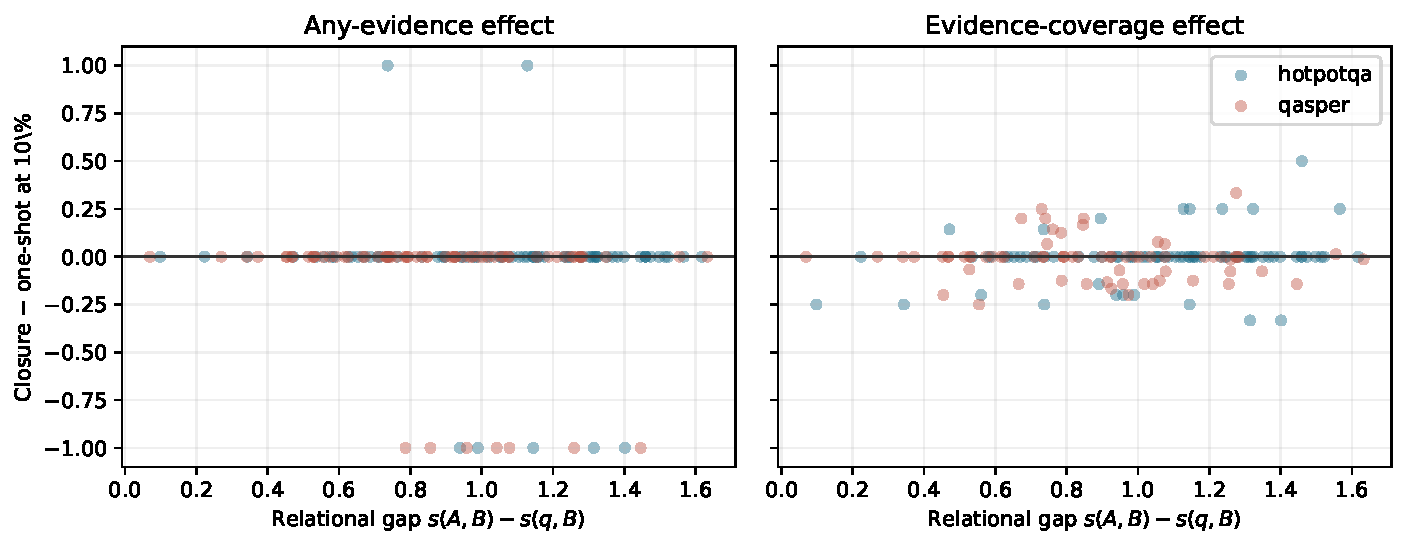
\includegraphics[width=0.92\linewidth]{../shared/results/paper2_5_iterative_pra/relational_gap_effect.pdf}
\caption{Paired $D=2$ minus one-shot effects at 10\%.  Relational gap does not predict a stable
closure advantage in the inherited semantic space.}
\label{fig:gap}
\end{figure}

\subsection{Search cost and full-K/V execution}

Figure~\ref{fig:cost} shows the compact-index cost.  At 10\%, $D=2$ uses 219.6 comparisons per
Hotpot example versus 50.1 one-shot (4.4$\times$), and 1395.9 versus 142.6 on QASPER
(9.8$\times$).  The higher QASPER multiplier follows from more candidates and larger frontiers.
These are exact comparison counts; wall time depends strongly on batching and hardware.

\begin{figure}[H]
\centering
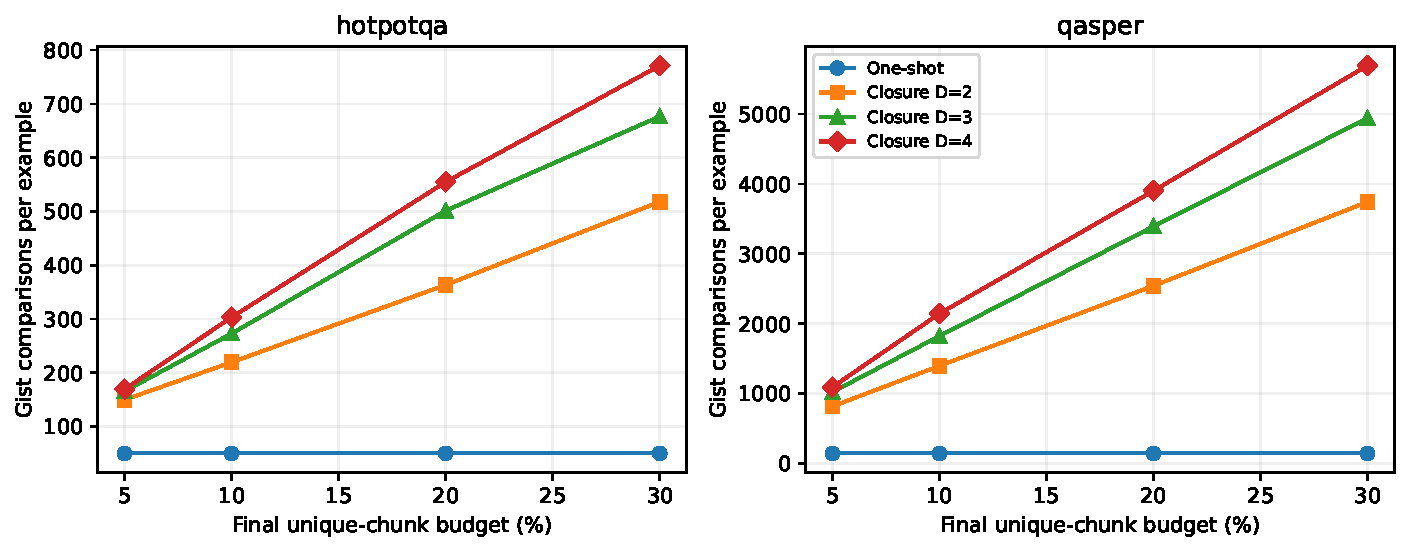
\includegraphics[width=0.92\linewidth]{../shared/results/paper2_5_iterative_pra/closure_search_cost.pdf}
\caption{Compact gist comparisons.  Iteration leaves final K/V budgets fixed but increases index
work with frontier size and depth.}
\label{fig:cost}
\end{figure}

The CUDA integration smoke materializes exactly three chunks and 96 K/V tokens for both methods.
Iterative routing takes 0.103/0.077 seconds on the Hotpot/QASPER examples, versus 0.107/0.073 for
one-shot in this trace-oriented implementation.  End-to-end times are 1.291/1.291 seconds for
closure and 1.304/1.347 seconds for one-shot.  The model records zero native-limit violations and
a maximum 64-token native operation.  These two cases validate the execution contract only.

\section{Discussion}

\subsection{What the experiments establish}

The synthetic result and the integration tests establish three mechanical facts.  First, a gist
can serve as a new query and recover a node that the root cannot afford at matched $B$.  Second,
deduplication, beam pruning, and hard budgets prevent exponential materialization.  Third, the
closure can remain entirely in compact routing state until final identities map to full native
K/V.

The natural-data result establishes a different boundary.  Paper 2's router learned an asymmetric
query--memory metric.  During iterative traversal, a memory-projected gist is reused as though it
were a valid query-projected representation.  Shared dimensionality does not imply shared
semantics.  Even without that asymmetry, evidence supervision optimized root-to-evidence ranking,
not evidence-to-next-evidence edges.  The mild Hotpot chain signal suggests some useful local
structure, but the any-recall loss, unstable budget trend, and relational-gap result show that it
is not yet a dependable graph.

The next experiment should therefore train a dual-use or explicitly compositional routing space.
Positive edges should connect an entry evidence chunk to the next required evidence chunk, while
hard negatives should include semantically related but relation-wrong chunks.  Evaluation must
remain matched-budget and include a shuffled-edge control.  A learned recurrent controller is
premature until that simpler geometry test succeeds.

\subsection{Relation to retrieval, agents, and recursive models}

Memory Networks repeatedly read differentiable memory to support multi-hop tasks, while RAG,
RETRO, and interleaved retrieval systems bring external evidence into generation
\cite{lewis2020rag,borgeaud2022retro,trivedi2023ircot}.  Agentic systems can reformulate a text
query after each model pass.  Iterative PRA is narrower: it traverses already computed latent
addresses inside one memory subsystem.  It avoids repeated text serialization and full-model
round trips, but it cannot replace an agent that must plan tools, verify evidence, or change the
retrieval language.

Tiny Recursive Models repeatedly transform internal latent and answer state
\cite{jolicoeurmartineau2025trm}.  Controlled autoregressive work finds no reliable gain from the
full autoregressive TRM architecture over simpler refinement baselines
\cite{rauba2026autoregressivetrm}.  Iterative PRA does not apply a tiny neural network repeatedly.
Its recurrence is $\textit{query}\rightarrow\textit{memory node}\rightarrow\textit{memory node}$.
This distinction motivates the parameter-free Level-1 test: retrieval recursion should earn its
complexity before neural state recursion is introduced.

\subsection{Paper 3 handoff}

Papers 1--2 conservatively compress search but materialize every selected chunk in full.  Iterative
closure produces more structure before transfer: hop, parent edges, direct relevance, path score,
confidence, branch entropy, and duplicate/overlap statistics.  The versioned graph keeps these
signals even when the final payload remains unchanged.  Paper 3 can therefore ask a separate
question: given a discovered closure, how much detail should each node receive?  This paper does
not test partial materialization.

\section{Limitations}

The held-out natural-data sample has 16 examples per dataset, repeated over five router seeds.
Seeds quantify projection sensitivity but do not create 80 independent questions.  Hotpot
evidence groups are source-contiguous spans, not annotated causal hop labels.  QASPER's selected
subset is yes/no and often one-group, so it tests direct retrieval more than multi-hop closure.

The inherited router is asymmetric.  Reusing memory-projected vectors as frontier queries is a
clean parameter-free probe, but it may be geometrically mismatched.  The experiment does not
include evidence-edge training, a learned update, a full agentic baseline, or Level-3 transformer-
conditioned traversal.  Downstream F1/EM is measured only in a two-example execution smoke and is
not used as evidence of quality.  Finally, the trace-oriented implementation launches many small
operations; production latency requires batched frontiers, batched examples, and a persistent
index service.

\section{Conclusion}

Bounded associative closure is a viable retrieval primitive when latent memory contains the
right edges.  It can find $B$ through $A$, preserve a graph explaining that discovery, and defer
full native K/V until search ends.  On controlled chains, that behavior is exact.  On the current
pretrained semantic geometry, however, the result is not yet strong enough to replace one-shot
PRA.  Hotpot shows a small chain-completion signal alongside semantic drift and substantially
more index work; QASPER favors direct retrieval.

The scientific lesson is specific.  Iterative machinery alone does not turn nearest-neighbor
embeddings into a relational graph.  The next step is to learn and falsify associative edges
directly, while retaining the same-budget baseline and the strict separation between compact
closure and native payload materialization.

\appendix
\section{Implementation Map}

The implementation is designed so another system can reproduce the mechanism without adopting
the entire PRA-HF package.  File and line references below refer to the accompanying source
revision.

\paragraph{Layer-local packed index.}
\texttt{src/pra\_hf/iterative.py:62--112} packs variable gist sets as
\texttt{[chunks,max\_gists,routing\_width]} plus a validity mask.  Records retain chunk identities
and payload handles, but packing copies no native K/V.

\paragraph{Graph contract.}
\texttt{iterative.py:115--170} defines node, edge, graph, and result records.  The JSON Schema is
\texttt{docs/papers/shared/schemas/retrieval\_graph\_v1.schema.json}.  Nodes retain direct score,
edge score, path score, hop, parents, winning gist, selection state, and materialization state.

\paragraph{Exact scoring and deterministic top-k.}
\texttt{iterative.py:203--224} normalizes frontier rows and computes
\texttt{einsum("fd,cgd->fcg")} before max reduction across gists.  A stable index tie-break is
applied before \texttt{torch.topk}, producing deterministic identities on CPU and CUDA.

\paragraph{Traversal.}
\texttt{iterative.py:226--412} performs root scoring, frontier expansion, anchoring, deduplication,
path pruning, Level-2 updates, stopping, and cost accounting.  The code never accesses
\texttt{chunk.token\_kv}.  Conversion at lines 422--443 returns selected payload handles only
after the graph is final.

\paragraph{Host-model integration.}
\texttt{src/pra\_hf/model.py:364--411} captures one root query with memory disabled, dispatches
one-shot or iterative routing, maps final identities to consumption layers, enables fixed memory,
and only then marks graph nodes materialized.  Generation thereafter uses the unchanged Paper 2
native-K/V path.

\paragraph{Reproduction.}
The experiment directory is \texttt{experiments/paper2\_5\_iterative\_pra/}.  Its
\texttt{run\_closure.py} file runs retrieval, \texttt{summarize\_results.py} derives figures,
and \texttt{run\_downstream\_smoke.py} checks CUDA integration.  Raw rows, tables, plots, and
graph JSONL are in the corresponding \texttt{shared/results/paper2\_5\_iterative\_pra/}
directory.

\section{Validation Gates}

The test suite checks $D=1$ equivalence to Top-$B$, deterministic batches, exact synthetic
two-hop recovery, deduplication and cycles, depth/beam/unique budgets, all path and frontier modes,
zero limits, layer locality, CPU/CUDA identity parity, and the no-materialization-before-closure
boundary.  The combined Qwen/Llama/Gemma/product/closure subset contains 83 passing tests.  The
full downstream smoke records zero native operation-limit violations.

\bibliographystyle{plain}
\bibliography{../shared/references}

\end{document}
